\lab{Pandas III: Grouping}{Pandas III: Grouping}
\objective{
Many data sets contain categorical values that naturally sort the data into groups.
Analyzing and comparing such groups is an important part of data analysis.
In this lab we explore pandas tools for grouping data and presenting tabular data more compactly, primarily through grouby and pivot tables.
}

\section*{Groupby} % ==========================================================

The file \texttt{mammal\_sleep.csv}\footnote{Proceedings of the National Academy of Sciences, 104 (3):1051--1056, 2007.
Updates from V. M. Savage and G. B. West, with additional variables supplemented by Wikipedia.
Available in \texttt{pydataset} (with a few more columns) under the key \texttt{"msleep"}.} contains data on the sleep cycles of different mammals, classified by order, genus, species, and diet (carnivore, herbivore, omnivore, or insectivore).
The \li{"sleep_total"} column gives the total number of hours that each animal sleeps (on average) every $24$ hours.
To get an idea of how many animals sleep for how long, we start off with a histogram of the \li{"sleep_total"} column.

\begin{lstlisting}
>>> import pandas as pd
>>> from matplotlib import pyplot as plt

# Read in the data and print a few random entries.
>>> msleep = pd.read_csv("mammal_sleep.csv")
>>> msleep.sample(5)
<<      name     genus   vore         order  sleep_total  sleep_rem  sleep_cycle
51  Jaguar  Panthera  carni     Carnivora         10.4        NaN          NaN
77  Tenrec    Tenrec   omni  Afrosoricida         15.6        2.3          NaN
10    Goat     Capri  herbi  Artiodactyla          5.3        0.6          NaN
80   Genet   Genetta  carni     Carnivora          6.3        1.3          NaN
33   Human      Homo   omni      Primates          8.0        1.9          1.5>>

# Plot the distribution of the sleep_total variable.
>>> msleep.plot(kind="hist", y="sleep_total", title="Mammalian Sleep Data")
>>> plt.xlabel("Hours")
\end{lstlisting}

\begin{figure}[H] % Mammal sleep_total hist (all groups)
    \centering
    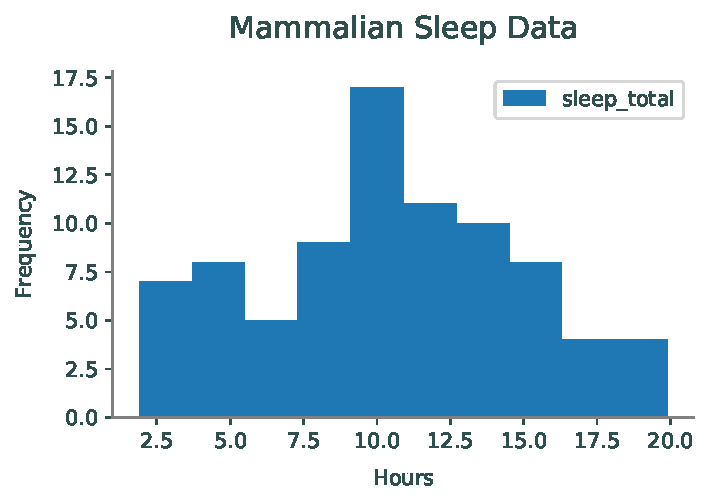
\includegraphics[width=.7\textwidth]{figures/mammal_hist.pdf}
    \caption{\li{"sleep_total"} frequencies from the mammalian sleep data set.}
    \label{fig:pandas-mammals-sleep-all}
\end{figure}

While this visualization is a good start, it doesn't provide any information about how different kinds of animals have different sleeping habits.
How long do carnivores sleep compared to herbivores?
Do mammals of the same genus have similar sleep patterns?

A powerful tool for answering these kinds of questions is the \li{groupby()} method of the pandas \li{DataFrame} class, which partitions the original \li{DataFrame} into groups based on the values in one or more columns.
The \li{groupby()} method does \textbf{not} return a new \li{DataFrame}; it returns a pandas \li{GroupBy} object, an interface for analyzing the original \li{DataFrame} by groups.

For example, the columns \li{"genus"}, \li{"vore"}, and \li{"order"} in the mammal sleep data all have a discrete number of categorical values that could be used to group the data.
Since the \li{"vore"} column has only a few unique values, we start by grouping the animals by diet.

\begin{lstlisting}
# List all of the unique values in the 'vore' column.
>>> set(msleep["vore"])
<<{nan, 'herbi', 'omni', 'carni', 'insecti'}>>

# Group the data by the 'vore' column.
>>> vores = msleep.groupby("vore")
>>> list(vores.groups)
<<['carni', 'herbi', 'insecti', 'omni']>>       # NaN values for vore were dropped.

# Get a single group and sample a few rows. Note vore='carni' in each entry.
>>> vores.get_group("carni").sample(5)
<<       name     genus   vore      order  sleep_total  sleep_rem  sleep_cycle
80    Genet   Genetta  carni  Carnivora          6.3        1.3          NaN
50    Tiger  Panthera  carni  Carnivora         15.8        NaN          NaN
8       Dog     Canis  carni  Carnivora         10.1        2.9        0.333
0   Cheetah  Acinonyx  carni  Carnivora         12.1        NaN          NaN
82  Red fox    Vulpes  carni  Carnivora          9.8        2.4        0.350>>
\end{lstlisting}

For starters, \li{groupby()} is useful for filtering a \li{DataFrame} by column values:
the command \li{df.groupby(col).get_group(value)} returns the rows of \li{df} where the entry of the \li{col} column is \li{value}.
The real advantage of \li{groupby()}, however, is how easy it makes it to compare groups of data.
Standard \li{DataFrame} methods like \li{describe()}, \li{mean()}, \li{std()}, \li{<<min>>()}, and \li{<<max>>()} all work on \li{GroupBy} objects to produce a new data frame that describes the statistics of each group.

\begin{lstlisting}
# Get averages of the numerical columns for each group.
>>> vores.mean()
<<         sleep_total  sleep_rem  sleep_cycle
vore
carni         10.379      2.290        0.373
herbi          9.509      1.367        0.418
insecti       14.940      3.525        0.161
omni          10.925      1.956        0.592>>

# Get more detailed statistics for 'sleep_total' by group.
>>> vores["sleep_total"].describe()
<<         count    mean    std  min   25%   50%     75%   max
vore
carni     19.0  10.379  4.669  2.7  6.25  10.4  13.000  19.4
herbi     32.0   9.509  4.879  1.9  4.30  10.3  14.225  16.6
insecti    5.0  14.940  5.921  8.4  8.60  18.1  19.700  19.9
omni      20.0  10.925  2.949  8.0  9.10   9.9  10.925  18.0>>
\end{lstlisting}

Multiple columns can be used simultaneously for grouping.
In this case, the \li{get_group()} method of the \li{GroupBy} object requires a tuple specifying the values for each of the grouping columns.

\begin{lstlisting}
>>> msleep_small = msleep.drop(["sleep_rem", "sleep_cycle"], axis=1)
>>> vores_orders = msleep_small.groupby(["vore", "order"])
>>> vores_orders.get_group(("carni", "Cetacea"))
<<                    name          genus   vore    order  sleep_total
30           Pilot whale  Globicephalus  carni  Cetacea          2.7
59       Common porpoise       Phocoena  carni  Cetacea          5.6
79  Bottle-nosed dolphin       Tursiops  carni  Cetacea          5.2>>
\end{lstlisting}

\subsection*{Visualizing Groups} % --------------------------------------------

There are a few ways that \li{groupby()} or similar techniques can simplify the process of visualizing groups of data.
First of all, \li{groupby()} makes it easy to visualize one group at a time.
The following visualization improve on Figure \ref{fig:pandas-mammals-sleep-all} by grouping mammals by their diets.

\begin{lstlisting}
# Plot histograms of 'sleep_total' for two separate groups.
>>> vores.get_group("carni").plot(kind="hist", y="sleep_total", legend="False",
                                                title="Carnivore Sleep Data")
>>> plt.xlabel("Hours")
>>> vores.get_group("herbi").plot(kind="hist", y="sleep_total", legend="False",
                                                title="Herbivore Sleep Data")
>>> plt.xlabel("Hours")
\end{lstlisting}

\begin{figure}[H] % Grouped mammal sleep_total histograms.
\captionsetup[subfigure]{justification=centering}
\centering
\begin{subfigure}{.495\textwidth}
    \centering
    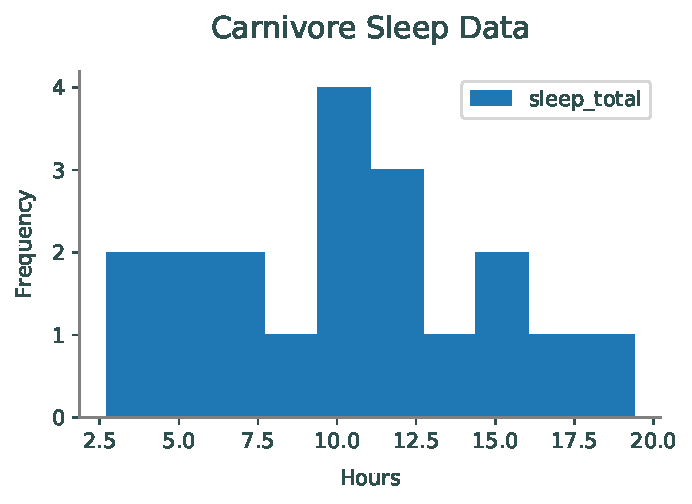
\includegraphics[width=\textwidth]{figures/mammal_hist_carni.pdf}
\end{subfigure}
%
\begin{subfigure}{.495\textwidth}
    \centering
    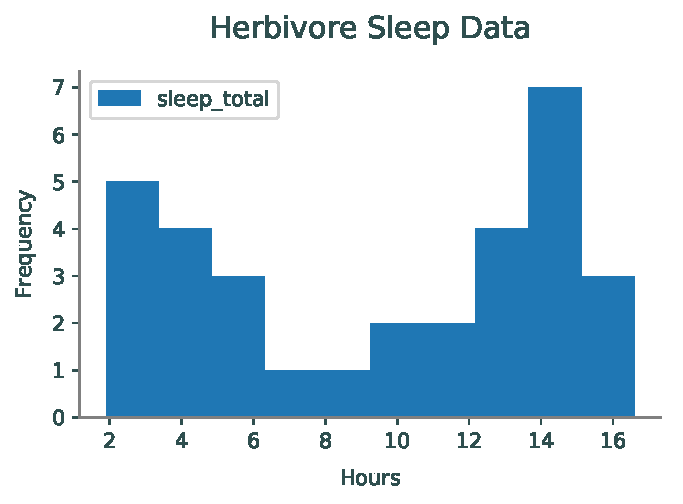
\includegraphics[width=\textwidth]{figures/mammal_hist_herbi.pdf}
\end{subfigure}
\caption{\li{"sleep_total"} histograms for two groups in the mammalian sleep data set.}
\end{figure}

\begin{comment} % hist() isn't a great option from a datavis standpoint.
\begin{info}
The \li{hist()} method of the \li{DataFrame} class has a keyword \li{by} that groups data before plotting, producing one histogram per group.
This can be a very quick way to get an overview of the data in multiple groups.

\begin{lstlisting}
>>> msleep.hist("sleep_total", by="vore", sharex=True)
>>> plt.tight_layout()
\end{lstlisting}
\end{info}
\end{comment}

The statistical summaries from the \li{GroupBy} object's \li{mean()}, \li{std()}, or \li{describe()} methods also lend themselves well to certain visualizations for comparing groups.

\begin{lstlisting}
>>> vores[["sleep_total", "sleep_rem", "sleep_cycle"]].mean().plot(kind="barh",
                xerr=vores.std(), title=r"Mammallian Sleep, $\mu\pm\sigma$")
>>> plt.xlabel("Hours")
>>> plt.ylabel("Mammal Diet Classification (vore)")
\end{lstlisting}

\begin{figure}[H]
    \centering
    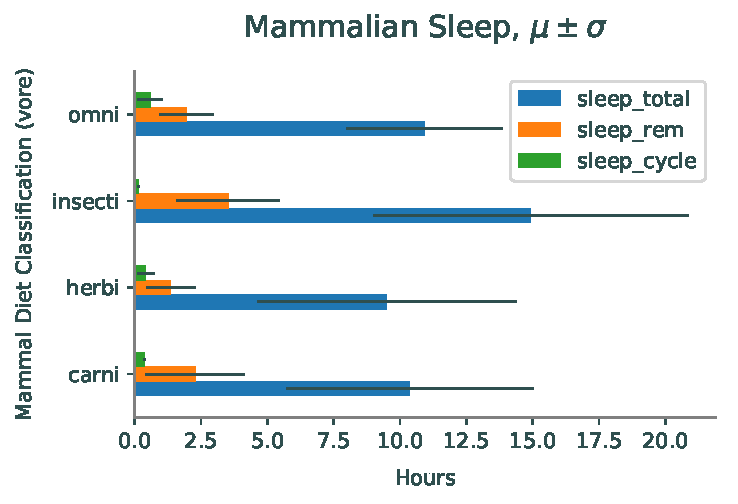
\includegraphics[width=.7\textwidth]{figures/mammal_bar.pdf}
\end{figure}

Box plots are well suited for comparing similar distributions.
The \li{boxplot()} method of the \li{GroupBy} class creates one subplot \textbf{per group}, plotting each of the columns as a box plot.

\begin{lstlisting}
# Use GroupBy.boxplot() to generate one box plot per group.
>>> vores.boxplot(grid=False)
>>> plt.tight_layout()
\end{lstlisting}

\begin{figure}[H]
    \centering
    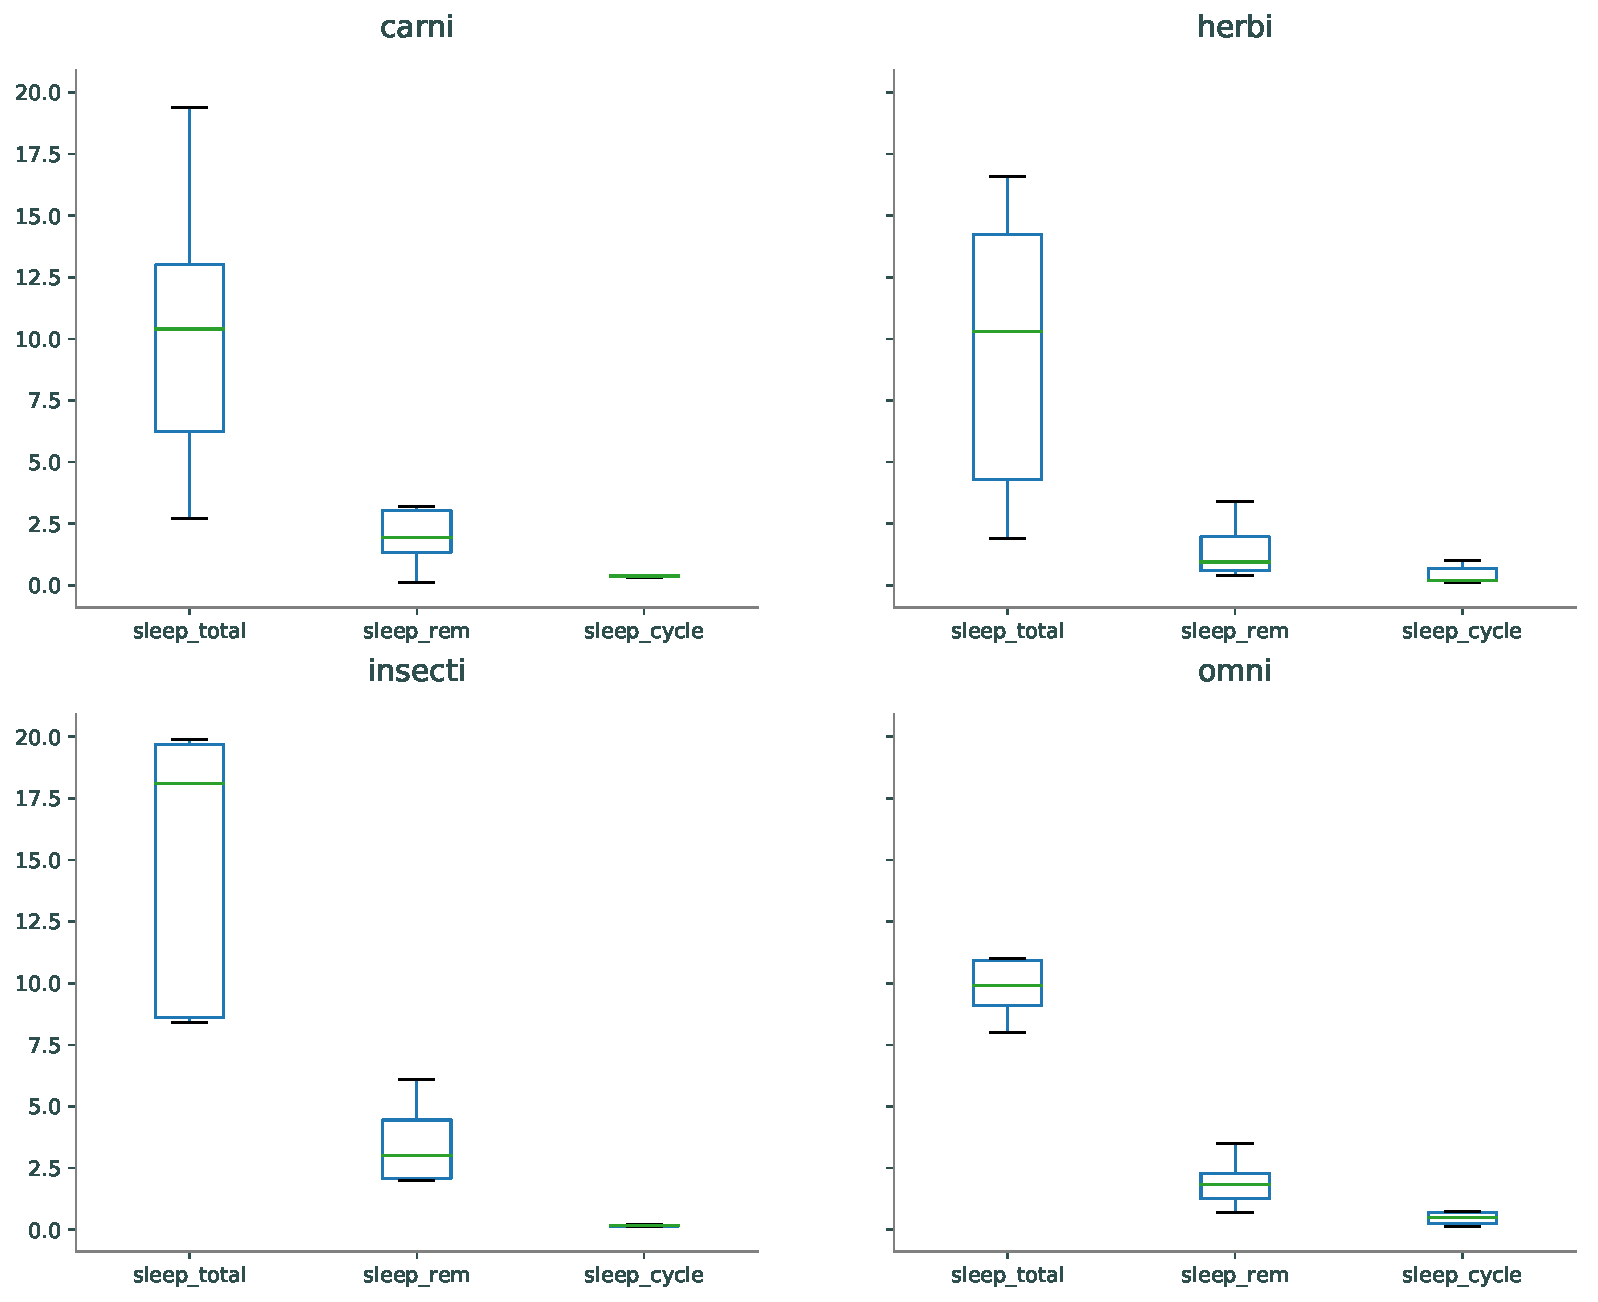
\includegraphics[width=.7\textwidth]{figures/mammal_box_groups.pdf}
\end{figure}

Alternatively, the \li{boxplot()} method of the \li{DataFrame} class creates one subplot \textbf{per column}, plotting each of the columns as a box plot.
Specify the \li{by} keyword to group the data appropriately.

\begin{lstlisting}
# Use DataFrame.boxplot() to generate one box plot per column.
>>> msleep.boxplot(["sleep_total", "sleep_rem"], by="vore", grid=False)
\end{lstlisting}

\begin{figure}[H]
    \centering
    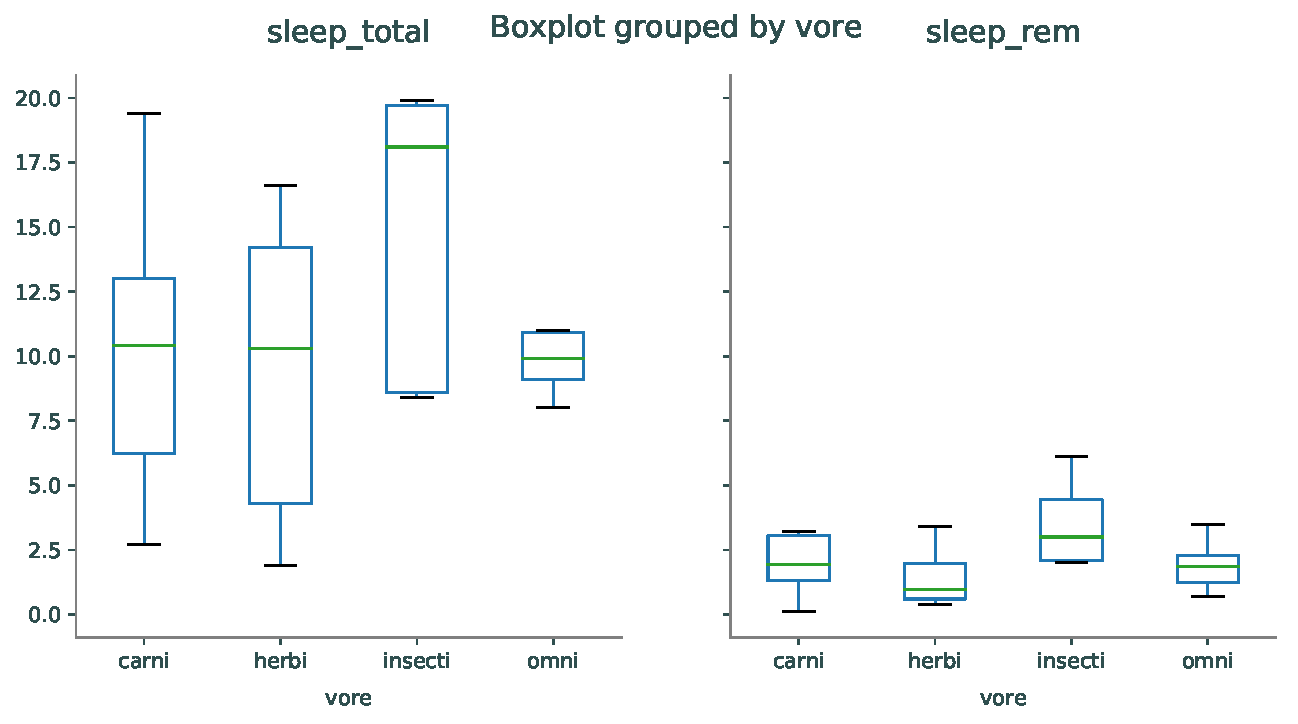
\includegraphics[width=.7\textwidth]{figures/mammal_box_cols.pdf}
\end{figure}

Like \li{groupby()}, the \li{by} argument can be a single column label or a list of column labels.
Similar methods exist for creating histograms (\li{GroupBy.hist()} and \li{DataFrame.hist()} with \li{by} keyword), but generally box plots are better for comparing multiple distributions.

\begin{problem} % More dataset visualizations.
Examine the following data sets from \li{pydataset} and answer the corresponding questions.
Use visualizations to support your conclusions.

\begin{itemize}
    \item \li{"iris"}, measurements of various species of iris flowers.
    \begin{enumerate}
        \item Which species is easiest to distinguish from the others? How?
        \item Given iris data without a species label, what strategies could you use to identify the flower's species?
    \end{enumerate}
    \item \li{"poisons"}, experimental results of three different poisons and four different treatments.
    \begin{enumerate}
        \item In general, which poison is most deadly?
        Which treatment is most effective?
        \item If you were poisoned, how would you choose the treatment if you did not know which poison it was? What if you did know which poison it was?
        \\(Hint: group the data by poison, then group each subset by treatment.)
    \end{enumerate}
    \item \li{"diamonds"}, prices and characteristics of almost 54,000 round-cut diamonds.
    \begin{enumerate}
        \item How does the color and cut of a diamond affect its price?
        \item Of the diamonds with color \li{"H"}, those with a \li{"Fair"} cut sell, on average, for a \textbf{higher} price than those with an \li{"Ideal"} (superior) cut.
        What other factors could explain this unintuitive statistic?
    \end{enumerate}
\end{itemize}
\end{problem}

\section*{Pivot Tables} % =====================================================

One of the downfalls of \li{groupby()} is that a typical \li{GroupBy} object has too much information to display coherently.
A \emph{pivot table} intelligently summarizes the results of a \li{groupby()} operation by aggregating the data in a specified way.
The standard tool for making a pivot table is the \li{pivot_table()} method of the \li{DataFrame} class.
As an example, consider the \li{"HairEyeColor"} data set from \li{pydataset}.

\begin{lstlisting}
>>> from pydataset import data
>>> hec = data("HairEyeColor")              # Load and preview the data.
>>> hec.sample(5)
<<     Hair    Eye     Sex  Freq
3     Red  Brown    Male    10
1   Black  Brown    Male    32
14  Brown  Green    Male    15
31    Red  Green  Female     7
21  Black   Blue  Female     9>>

>>> for col in ["Hair", "Eye", "Sex"]:      # Get unique values per column.
...     print("{}: {}".format(col, ", ".join(set(str(x) for x in hec[col]))))
...
Hair: Brown, Black, Blond, Red
Eye: Brown, Blue, Hazel, Green
Sex: Male, Female
\end{lstlisting}

There are several ways to group this data with \li{groupby()}.
However, since there is only one entry per unique hair-eye-sex combination, the data can be completely presented in a pivot table.

\begin{lstlisting}
>>> hec.pivot_table(values="Freq", index=["Hair", "Eye"], columns="Sex")
<<Sex          Female  Male
Hair  Eye
Black Blue        9    11
      Brown      36    32
      Green       2     3
      Hazel       5    10
Blond Blue       64    30
      Brown       4     3
      Green       8     8
      Hazel       5     5
Brown Blue       34    50
      Brown      66    53
      Green      14    15
      Hazel      29    25
Red   Blue        7    10
      Brown      16    10
      Green       7     7
      Hazel       7     7>>
\end{lstlisting}

Listing the data in this way makes it easy to locate data and compare the female and male groups.
For example, it is easy to see that brown hair is more common than red hair and that about twice as many females have blond hair and blue eyes than males.

Unlike \li{"HairEyeColor"}, many data sets have more than one entry in the data for each grouping (for example, if there were two or more rows in the original data for females with blond hair and blue eyes).
To construct a pivot table, data of similar groups must be \emph{aggregated} together in some way.
By default entries are aggregated by averaging the non-null values.
Other options include taking the min, max, standard deviation, or just counting the number of occurrences.

As an example, consider again the Titanic data set found in \texttt{titanic.csv}\footnote{There is a \texttt{"Titanic"} data set in \texttt{pydataset}, but it does not contain as much information as the data in \texttt{titanic.csv}.}.
For this analysis, take only the \li{"Survived"}, \li{"Pclass"}, \li{"Sex"}, \li{"Age"}, \li{"Fare"}, and \li{"Embarked"} columns, replace null age values with the average age, then drop any rows that are missing data.
To begin, we examine the average survival rate grouped by sex and passenger class.

\begin{lstlisting}
>>> titanic = pd.read_csv("titanic")
>>> titanic = titanic[["Survived", "Pclass", "Sex", "Age", "Fare", "Embarked"]]
>>> titanic["Age"].fillna(titanic["Age"].mean(), inplace=True)
>>> titanic.dropna(inplace=True)

>>> titanic.pivot_table(values="Survived", index="Sex", columns="Pclass")
<<Pclass    1.0    2.0    3.0
Sex
female  0.965  0.887  0.491
male    0.341  0.146  0.152>>
\end{lstlisting}

\begin{info} % pivot_table() is a shortcut for a complicated groupby().
The \li{pivot_table()} method is just a convenient way of performing a potentially complicated \li{groupby()} operation with aggregation and some reshaping.
For example, the following code is equivalent to the previous example.

\begin{lstlisting}
>>> titanic.groupby(["Sex", "Pclass"])["Survived"].mean().unstack()
<<Pclass    1.0    2.0    3.0
Sex
female  0.965  0.887  0.491
male    0.341  0.146  0.152>>
\end{lstlisting}

The \li{stack()}, \li{unstack()}, and \li{pivot()} methods provide more advanced shaping options.
\end{info}

Among other things, this pivot table clearly shows how much more likely females were to survive than males.
To see how many entries fall into each category, or how many survived in each category, aggregate by counting or summing instead of taking the mean.

\begin{lstlisting}
# See how many entries are in each category.
>>> titanic.pivot_table(values="Survived", index="Sex", columns="Pclass",
...                     aggfunc="count")
<<Pclass  1.0  2.0  3.0
Sex
female  144  106  216
male    179  171  493>>

# See how many people from each category survived.
>>> titanic.pivot_table(values="Survived", index="Sex", columns="Pclass",
...                     aggfunc="sum")
<<Pclass    1.0   2.0    3.0
Sex
female  137.0  94.0  106.0
male     61.0  25.0   75.0>>
\end{lstlisting}

\subsection*{Discretizing Continuous Data} % ----------------------------------

So far we have examined survival rates based on sex and passenger class.
Another factor that could have played into survival is age.
Were male children as likely to die as females in general?
We can investigate this question by \emph{multi-indexing}, or pivoting on more than just two variables, by adding in another index.

In the original dataset, the \li{"Age"} column has a floating point value for the age of each passenger.
If we just added \li{"Age"} as another pivot, then the table would create a new row for \textbf{each} age present.
Instead, we partition the \li{"Age"} column into intervals with \li{pd.cut()}, thus creating a categorical that can be used for grouping.

\newpage

\begin{lstlisting}
# pd.cut() maps continuous entries to discrete intervals.
>>> pd.cut([6, 1, 2, 3, 4, 5, 6, 7], [0, 4, 8])
<<[(0, 4], (0, 4], (0, 4], (0, 4], (4, 8], (4, 8], (4, 8], (0, 4]]
Categories (2, interval[int64]): [(0, 4] < (4, 8]]>>

# Partition the passengers into 3 categories based on age.
>>> age = pd.cut(titanic['Age'], [0, 12, 18, 80])

>>> titanic.pivot_table(values="Survived", index=["Sex", age],
                        columns="Pclass", aggfunc="mean")
<<Pclass             1.0    2.0    3.0
Sex    Age
female (0, 12]   0.000  1.000  0.467
       (12, 18]  1.000  0.875  0.607
       (18, 80]  0.969  0.871  0.475
male   (0, 12]   1.000  1.000  0.343
       (12, 18]  0.500  0.000  0.081
       (18, 80]  0.322  0.093  0.143>>
\end{lstlisting}

From this table, it appears that male children (ages 0 to 12) in the 1st and 2nd class were very likely to survive, whereas those in 3rd class were much less likely to.
This clarifies the claim that males were less likely to survive than females.
However, there are a few oddities in this table: zero percent of the female children in 1st class survived, and zero percent of teenage males in second class survived.
To further investigate, count the number of entries in each group.

%
% This might seem a little odd, but if we looked at our data set again to see how many passengers fell into this category of female, 1st class, and age 0 to 12, we would find only one passenger.
% Therefore, the statistic that 0\% of female children in first class lived is misleading.

\begin{lstlisting}
>>> titanic.pivot_table(values="Survived", index=["Sex", age],
                        columns="Pclass", aggfunc="count")
<<Pclass           1.0  2.0  3.0
Sex    Age
female (0, 12]     1   13   30
       (12, 18]   12    8   28
       (18, 80]  129   85  158
male   (0, 12]     4   11   35
       (12, 18]    4   10   37
       (18, 80]  171  150  420>>
\end{lstlisting}

This table shows that there was only 1 female child in first class and only 10 male teenagers in second class, which sheds light on the previous table.

\begin{warn}
The previous pivot table brings up an important point about partitioning datasets.
The Titanic dataset includes data for about 1300 passengers, which is a somewhat reasonable sample size, but half of the groupings include less than 30 entries, which is \textbf{not} a healthy sample size for statistical analysis.
Always carefully question the numbers from pivot tables before making any conclusions.
\end{warn}

Pandas also supports multi-indexing on the columns.
As an example, consider the price of a passenger tickets.
This is another continuous feature that can be discretized with \li{pd.cut()}.
Instead, we use \li{pd.qcut()} to split the prices into 2 equal quantiles.
Some of the resulting groups are empty; to improve readability, specify \li{fill_value} as the empty string or a dash.

\begin{lstlisting}
# pd.qcut() partitions entries into equally populated intervals.
>>> pd.qcut([1, 2, 5, 6, 8, 3], 2)
<<[(0.999, 4.0], (0.999, 4.0], (4.0, 8.0], (4.0, 8.0], (4.0, 8.0], (0.999, 4.0]]
Categories (2, interval[float64]): [(0.999, 4.0] < (4.0, 8.0]]>>

# Cut the ticket price into two intervals (cheap vs expensive).
>>> fare = pd.qcut(titanic["Fare"], 2)
>>> titanic.pivot_table(values="Survived",
                        index=["Sex", age], columns=[fare, "Pclass"],
                        aggfunc="count", fill_value='-')
<<Fare            (-0.001, 14.454]          (14.454, 512.329]
Pclass                       1.0 2.0  3.0               1.0 2.0 3.0
Sex    Age
female (0, 12]                 -   -    7                 1  13  23
       (12, 18]                -   4   23                12   4   5
       (18, 80]                -  31  101               129  54  57
male   (0, 12]                 -   -    8                 4  11  27
       (12, 18]                -   5   26                 4   5  11
       (18, 80]                8  94  350               163  56  70>>
\end{lstlisting}

Not surprisingly, most of the cheap tickets went to passengers in 3rd class.
%
% It should be noted though that with datasets where NaN's occur frequently, some preprocessing needs to be done so as to get the most accurate statistics and insights about your dataset.

\begin{problem} % More Titanic analysis.
Suppose that someone claims that the city from which a passenger embarked had a strong influence on the passenger's survival rate.
Investigate this claim.
\begin{enumerate}
    \item Check the survival rates of the passengers based on where they embarked from (given in the \li{"Embarked"} column).
    \item Create a pivot table to examine survival rates based on both place of embarkment and gender.
    \item What do these tables suggest to you about the significance of where people embarked in influencing their survival rate?
    Examine the context of the problem, and explain what you think this really means.
    \item Investigate the claim further with at least two more pivot tables, exploring other criteria (e.g., class, age, etc.).
    Carefully explain your conclusions.
\end{enumerate}
\end{problem}

\newpage

\begin{problem} % More grouping visualizations / pivot tables.
Examine the following data sets from \li{pydataset} and answer the corresponding questions.
Use visualizations and/or pivot tables as appropriate to support your conclusions.
\begin{itemize}
    \item \li{"npk"}, an experiment on the effects of nitrogen (N), phosphate (P), and potassium (K) on the growth of peas.
    \begin{enumerate}
        \item Which element is most effective in general for simulating growth?
        Which is the least effective?
        \item What combination of N, P, and K is optimal? What combination is the worst?
    \end{enumerate}
    \item \li{"swiss"}, standardized fertility measures and socio-economic indicators for French-speaking provinces of Switzerland at about 1888.
    \begin{enumerate}
        \item What is the relationship in the data between fertility rates and infant mortality?
        \item How are provinces that are predominantly Catholic different from non-Catholic provinces, if at all?
        \item What factors in the data are the most important for predicting fertility?
    \end{enumerate}
    \item Examine a data set of your choice.
    Formulate simple questions about the data and hypothesize the answers to those questions.
    Demonstrate the correctness of incorrectness of each hypothesis.
    Explain your conclusions.
\end{itemize}
\end{problem}
